\begin{document}
\title {\ZHH \huge git使用}
\author {\small gaccob}
\date {\small 2013 年 5 月 21 日}
\maketitle

{\ZHH git的示意图}\par
\begin{figure}[htbp]
    \centering
    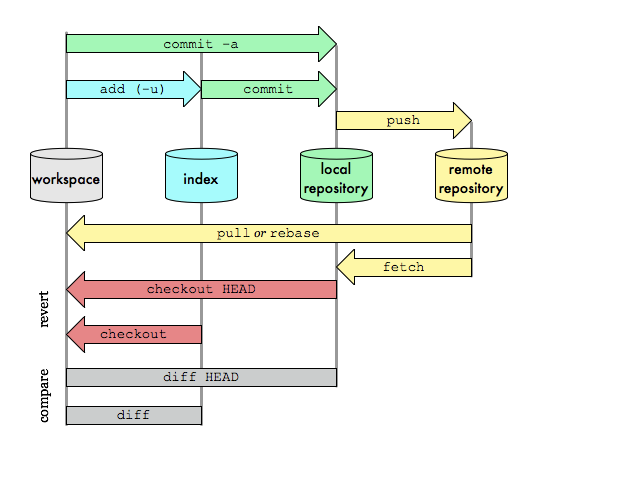
\includegraphics[width=300pt, keepaspectratio]{git.png}
\end{figure}
\vspace{10pt}


{\ZHH git的配置}\par
\begin{lstlisting}[language=bash]
    # `\color{gray} 当前用户的git配置, 一般保存在\$HOME/.gitconfig中`
    git config --global

    # `\color{gray} 系统的git配置, 一般保存在/etc/gitconfig中`
    git config --system

    # `\color{gray} 查看所有配置信息`
    git config --list

    # `\color{gray} 配置用户名`
    git config --global user.name gaccob
    git config --global user.name gaccob@qq.com

    # `\color{gray} 配置git的编辑器`
    git config --global core.editor vim
\end{lstlisting} \par
\vspace{10pt}


{\ZHH git的基本使用}\par
\begin{lstlisting}[language=bash]
    # `\color{gray} 拉取代码`
    git clone repo-git

    # `\color{gray} 检查代码仓库路径`
    git remote -v

    # `\color{gray} 建立分支`
    git branch branch-name

    # `\color{gray} 切换分支`
    git checkout branch-name

    # `\color{gray} 查看本地的修改`
    git diff head file-name

    # `\color{gray} 提交修改到本地仓库`
    git commit

    # `\color{gray} 提交本地的commit到远程仓库`
    git push origin head

    # `\color{gray} 增加修改到上次commit`
    git commit -s --amend

    # `\color{gray} 查看最近n次的git记录`
    git log -n

    # `\color{gray} 查看最近一次的git统计记录`
    git log -1 --stat

    # `\color{gray} 查看某次提交的git统计记录`
    git show hash --stat

    # `\color{gray} 查看某个文件的提交记录`
    git log --pretty=oneline file-name

    # `\color{gray} 查看某个文件的某次修改`
    git show hash file-name

    # `\color{gray} rebase到某分支, 如果有冲突, 解决之后再continue`
    git rebase branch-name
    git rebase --continue

    # `\color{gray} 如果放弃本次修改, 可以直接checkout到上一次commit, 或者reset`
    git checkout file-name
    git reset --hard
\end{lstlisting}
\vspace{10pt}


{\ZHH git的其他tips}\par
{如果要合并最近几次的commit, 找到需要合并的记录的上一条id, git rebase -i id, 在出现的列表中, 最上面的选择pick, 其余squash就可以了. }\par
{如果在分支中, 不commit而rebase代码, 可会有冲突, 这时候可以git stash, git pull, git stash pop. }

\end{document}
